%!TEX root = /Users/stevenmartell1/Documents/iSCAM-project/docs/iSCAM-guide/BeamerGuide/overView.tex


\section[Compiling]{Compiling Source Code} % (fold)
\label{sec:compiling_source_code}

\begin{frame}
	\frametitle{Compiling ADMB source code}
	What you need:
	\begin{itemize}
		\item C++ compiler (gcc recommended)
		\begin{itemize}
			\item Mac OSX: install Xcode from appstore
			\item Linux: \url{http://gcc.gnu.org/}
			\item Windoze: \url{http://www.mingw.org/}
		\end{itemize}
		\item ADMB libraries: \url{http://admb-project.org/downloads}
	\end{itemize}
	\vfill
	ADMB source code for \iscam\ found in:\\
	\texttt{./iSCAM-trunk/src/admb-code/}
\end{frame}

\begin{frame}
	\frametitle{Compiling from the command line}
	At the command line:
	\begin{itemize}[<+->]
		\item use cd to navigate to the ./iSCAM-trunk directory
		\item \underline{Linux or Mac OSX:} type Make
		\item \underline{Windows:} see \url{http://gnuwin32.sourceforge.net/packages/make.htm}
	\end{itemize}
	
	\only<1>{
	\vspace{-.25in}
	\begin{figure}[htbp]
		\centering
			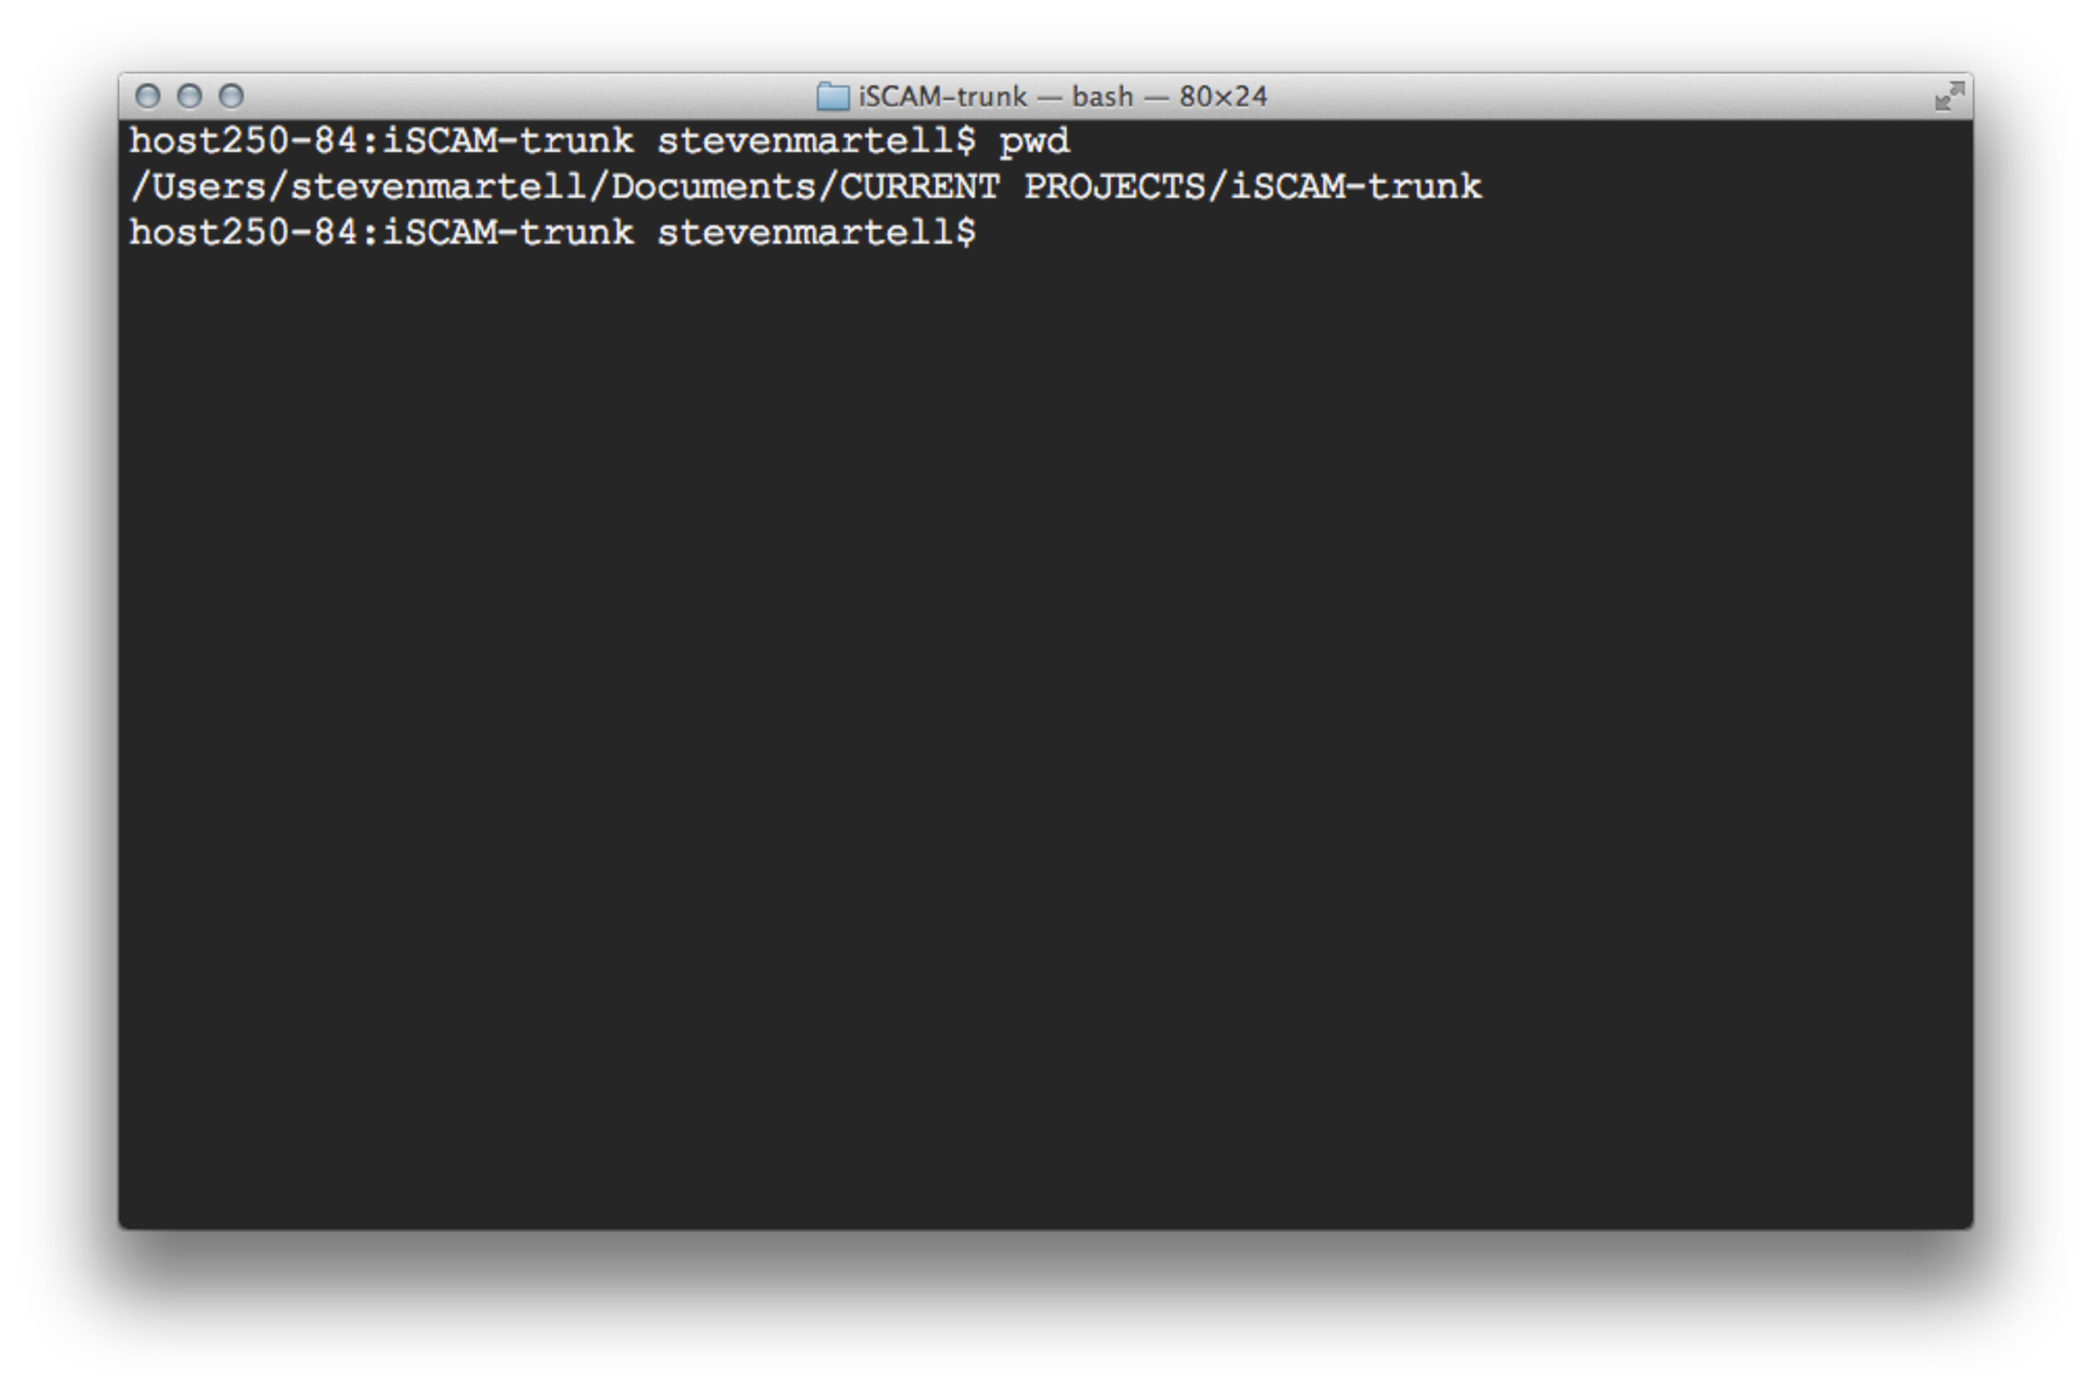
\includegraphics[height=2.5in]{screenCaptures/Term_iSCAM-trunk.pdf}
		\caption{}
		\label{fig:screenCaptures_Term_iSCAM-trunk}
	\end{figure}
	}
	\only<2>{
	\vspace{-.25in}
	\begin{figure}[htbp]
		\centering
			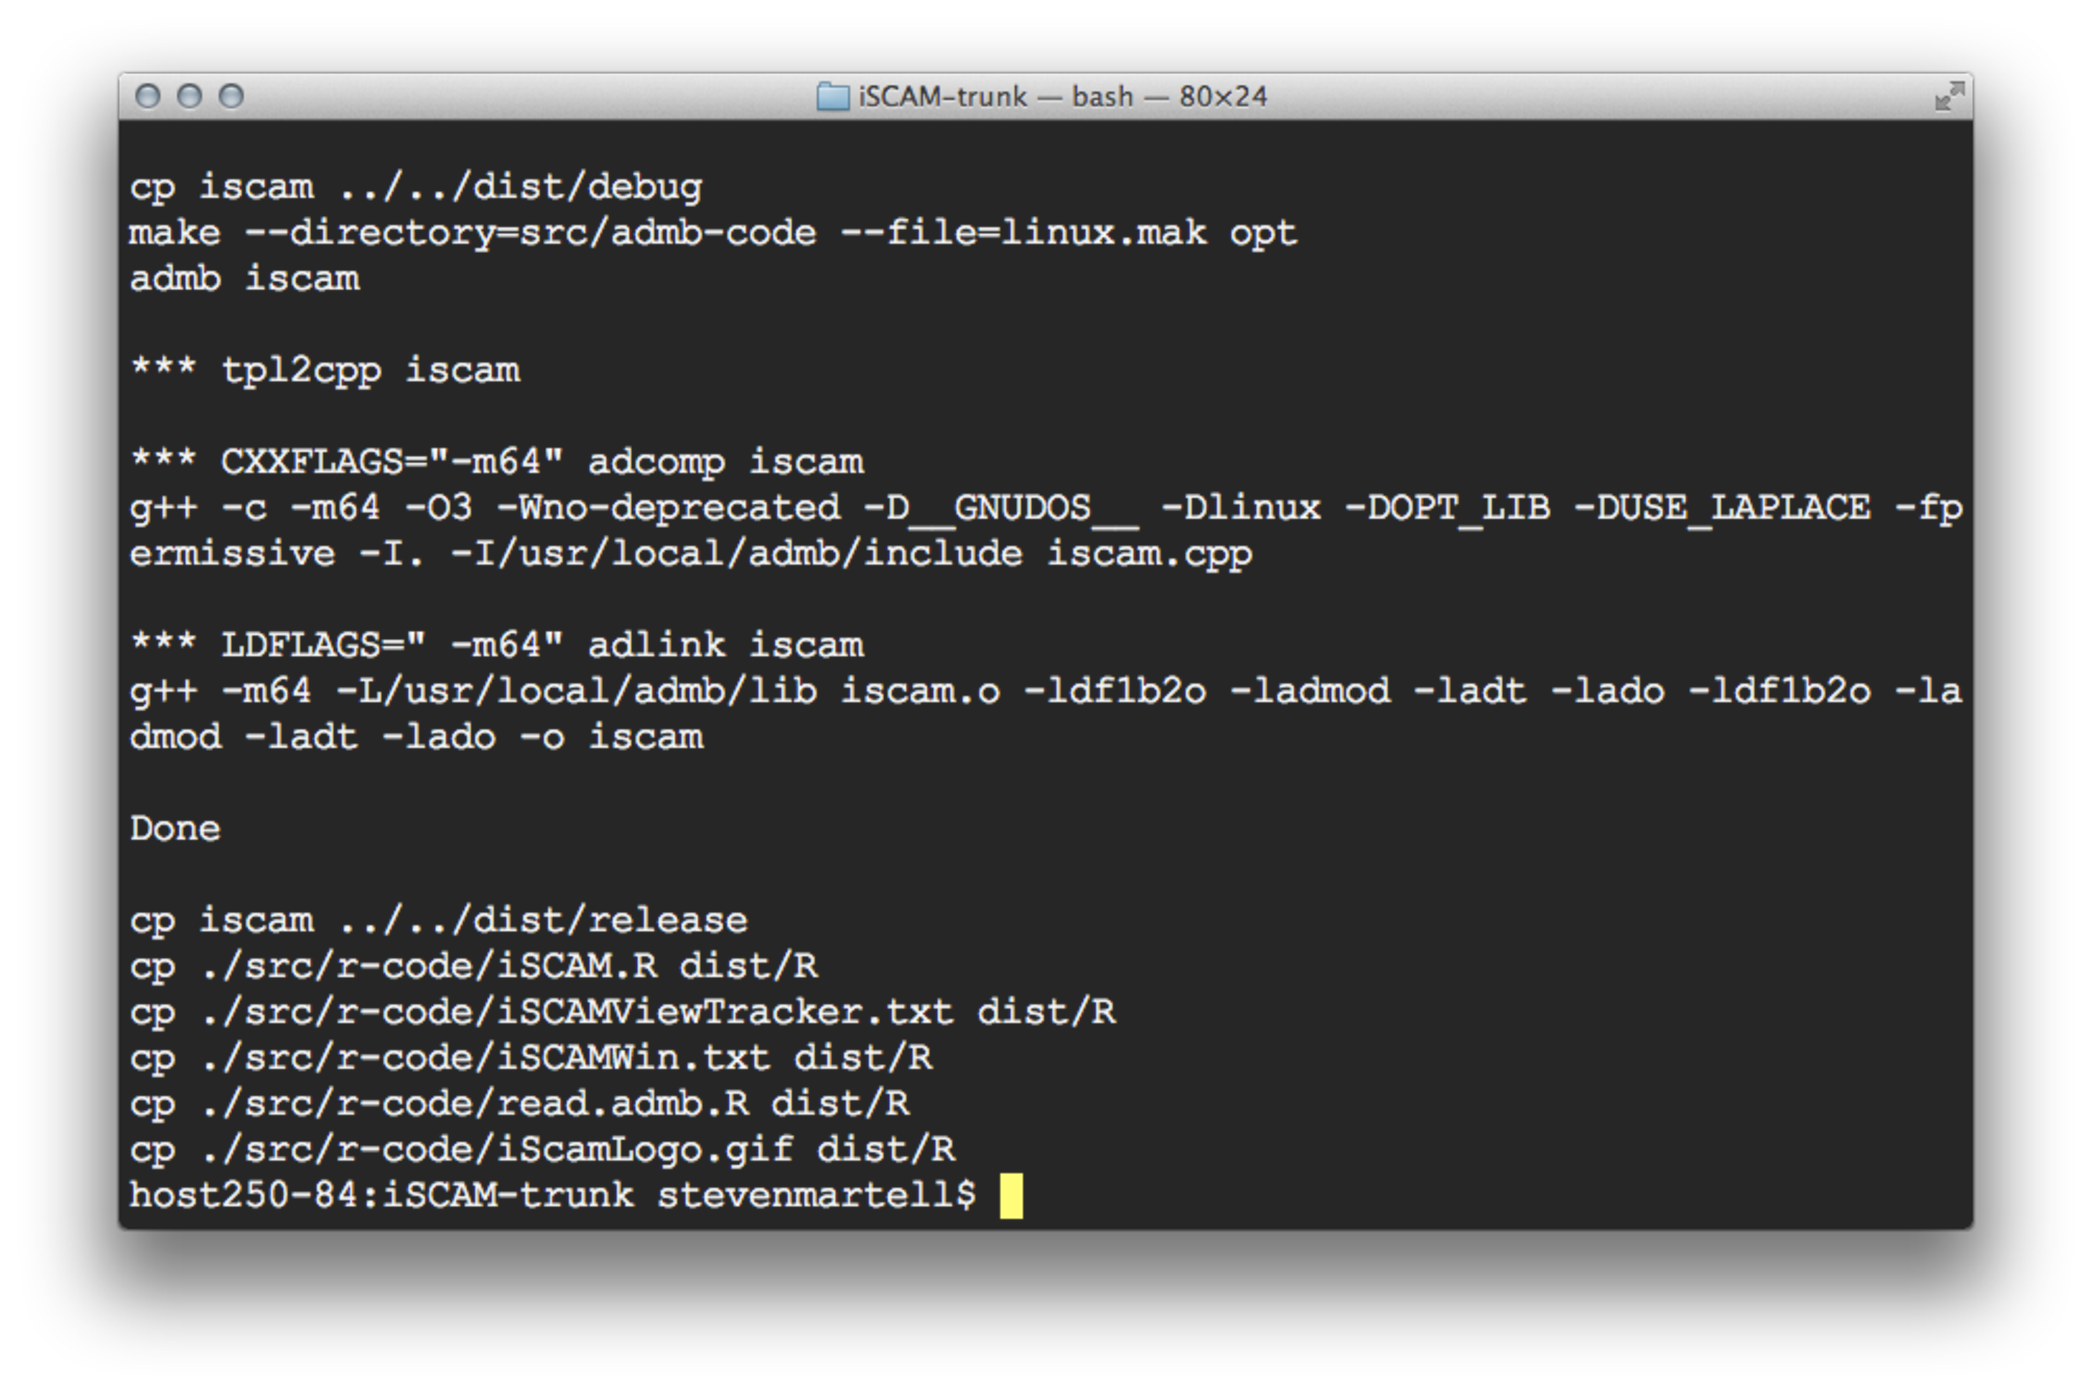
\includegraphics[height=2.5in]{screenCaptures/Term_make.pdf}
		\caption{}
		\label{fig:screenCaptures_Term_make}
	\end{figure}
	}
	\only<3>{
	\vspace{0.25in}
	Using the make file will compile the \iscam\ source code and place copies of the code in the distribution directory ("dist")
	}
\end{frame}

\begin{frame}
	\frametitle{Using make on windoze machines}
	If you want to run makefiles on Windows that were written for Mac or Linux, you need to reinstall mingw.  Make sure to check off "Developer tools" and "C++ libraries" and "Objective C libraries".  Then run the mingw shell from the start menu and once inside that you can just type "make" as usual.
\end{frame}

\begin{frame}[fragile]
	\frametitle{Windoze, c/o Gerry Black}
	Download Cygwin from \url{http://cygwin.com/setup.exe}  (don't use the 1st site listed)

	During the install do the default install, except also include the developer folder.

	Run the cygwin cmd prompt, and then do the export below…

	OR Adam Cook found that using doing the following in MinGW also works.

	\begin{verbatim}
	 $export ADMB_HOME="C:\Program Files\ADMB-11"
	 
	 $cd ~/iscam-project/src/admb-code
	 
	 $make
	 
	 $cd ~/iscam-project/examples/ECODETECTIVE/DATA
	 
	 $make
	\end{verbatim}	
\end{frame}

% section compiling_source_code (end)

